\documentclass[a4paper]{jsarticle}
\usepackage[dvipdfmx]{graphicx}
\usepackage{amsmath}
\usepackage{bm}
\renewcommand{\thesection}{第\arabic{section}問}
\renewcommand{\thesubsection}{(\arabic{subsection})}
\renewcommand{\thesubsubsection}{(\alph{subsubsection})}
\begin{document}

\title{2013分野3}
\author{nakao}
\maketitle

\section{}
\subsection{}
\subsubsection{}
断面平均流速を$v$とすると、
\begin{equation}
  E = \frac{v^2}{2g} + h
\end{equation}
が成り立つ。連続式
$Q = v b h$により、
\begin{equation}
  E = \frac{Q^2}{2 g b^2 h^2} + h
\end{equation}
となる。

\subsubsection{}
式(2)より、
\begin{equation}
  \left(\frac{Q^2}{b^2}\right)^2 = 2 g h^2 (E -h)
\end{equation}
となるから、
\begin{equation}
  f(h) = 2 g h^2 (E - h)
\end{equation}
である。
$f^{\prime}(h) = 0$を解いて
$h = \frac{2}{3} E$を得る。

\subsubsection{}
$Q = b \sqrt{f(h)}$より、$f(h)$が最大のときに$Q$が最大になる。
$h = \frac{2}{3}E$とすれば$f(h)$が最大になり、
\begin{equation}
  Q_{max} = b \sqrt{f \left(\frac{2}{3}E\right)}
  = b \sqrt{\frac{8}{27} g E^3}
\end{equation}
である。このとき断面Bにおける流速と水深をそれぞれ
$v_B, h_B$とすると、
\begin{equation}
  v_B h_B \frac{b}{2} = Q_{max} 
\end{equation}
であることから
\begin{equation}
  v_B = \frac{4}{3 h_B} \sqrt{\frac{2 g E^3}{3}}
\end{equation}
を得る。

\subsubsection{}
比エネルギーの保存則
\begin{equation}
  \frac{\mathrm{d} E}{\mathrm{d} x}
  = \frac{\mathrm{d}}{\mathrm{d} x}
  \left(\frac{Q^2}{2 g b^2 h^2} + h\right)
  = 0
\end{equation}
を展開すると、
\begin{equation}
  \frac{\mathrm{d} h}{\mathrm{d} x}
  = \frac{\mathrm{Fr^2}}{1 - \mathrm{Fr^2}}
  \frac{\mathrm{d} B}{\mathrm{d} x}
\end{equation}
が得られる。$\mathrm{Fr}$はフルード数である。
比エネルギーが保存するためには跳水が起こらないことが必要であり、
流下方向に常流か射流かは変化しない。
したがって、$1 - \mathrm{Fr}^2$の符号は流下方向に変化しない。
常流と射流のそれぞれの場合について、水面形は図1の通り。
\begin{figure}[htb]
  \centering
  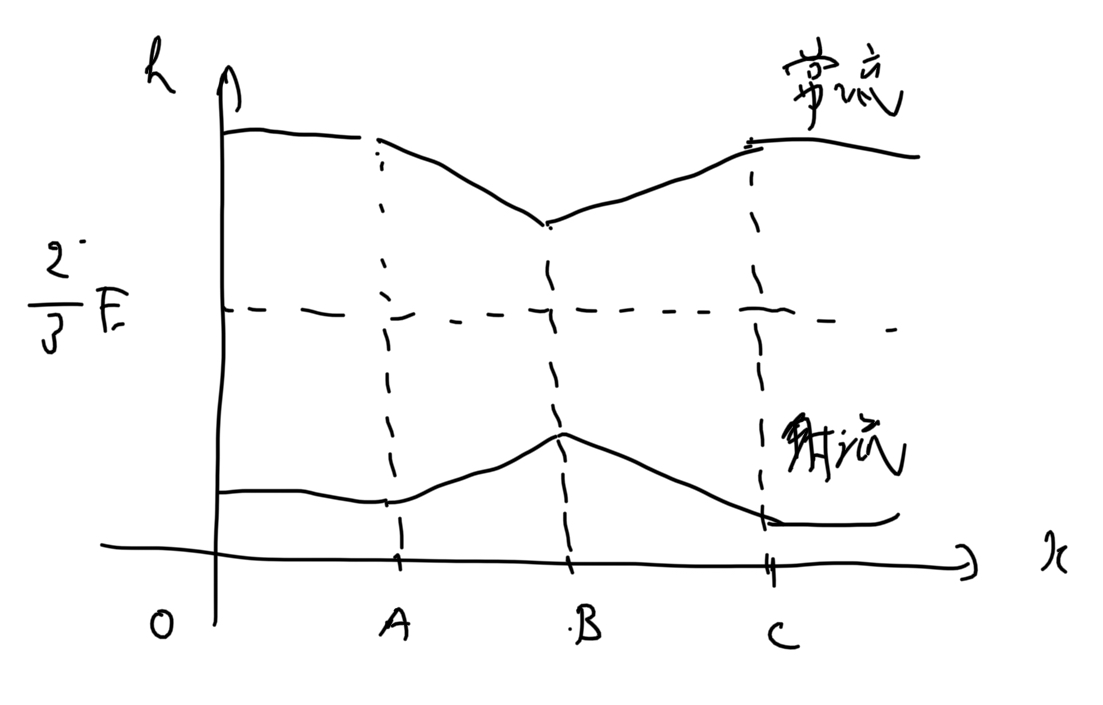
\includegraphics[width=0.5\hsize]{fig1.png}
  \caption{常流または射流のときの水面形}
\end{figure}

\subsection{}
\subsubsection{}
エネルギーフラックス$F$を表す式で各項の積分を計算すると、
\begin{align}
  \overline{\int_{-h}^0 \rho g z u \mathrm{d} z}
  &= -\frac{1}{2} a \rho \sqrt{g^3 h^3} \overline{\cos (kx - \omega t)}
  = 0 \\
  \overline{\int_{-h}^0 \frac{\rho}{2} u^3 \mathrm{d} z}
  &= \frac{1}{8} \rho a^3 \sqrt{\frac{g^3}{h}}
  (\overline{\cos 3(k x \omega t)} + 3 \overline{\cos (k x - \omega t)}) = 0 \\
  \overline{\int_{-h}^0 p u \mathrm{d} z}
  &= \frac{1}{2} \rho a \sqrt{g^3 h} (a + a \overline{\cos 2(k x - \omega t)} + h \overline{\cos (k x - \omega t)})
  = \frac{1}{2} \rho a^2 \sqrt{g^3 h}
\end{align}
であり、
\begin{equation}
  F = \overline{\int_{-h}^0 \left(\rho g z + \frac{\rho}{2} u^2\right) \mathrm{d} z}
  + \overline{\int_{-h}^0 p u \mathrm{d} z}
  = \frac{1}{2} \rho a^2 \sqrt{g^3 h}
\end{equation}
を得る。

\subsubsection{}
断面Bにおける波の振幅を$a_B$とすると、エネルギーフラックスが一定であるから、
\begin{equation}
  \frac{1}{2} \rho a^3 \sqrt{g^3 h} b
  = \frac{1}{2} \rho a_B^3 \sqrt{g^3 h} \frac{b}{2}
\end{equation}
が成り立つ。したがって、
\begin{equation}
  a_B = 2^{\frac{1}{3}} a
\end{equation}
である。
\end{document}